\section{Methodology}
\label{sec:methodology}

\subsection{Architecture of the framework}
\label{sec:architecture}

Figure~\ref{fig:architecture} shows how the study is assembled, in five
stages. A corpus of prompts from four task families is selected and split
(Section~\ref{sec:datasets}). Each prompt is then run through every cell of a
model-size by reasoning-mode grid on one GPU, while board power is sampled and
integrated over measurement windows and the answers are graded
(Section~\ref{sec:setup}). Joining grades and costs gives a label table, from
which routers learn to predict which cells succeed, and a threshold turns those
predictions into a choice of cell (Section~\ref{sec:routers}). Manual
escalation policies and routed policies are then charged by one cost function,
with the router's own tokens, latency and energy added for the routed ones
(Sections~\ref{sec:tax} and \ref{sec:net}), and the outputs are the escalation
tax, joules per solved prompt, net saving and carbon. The same policy and tax
code is finally applied to a public table of per-query outcomes and to a hosted
ladder, neither of which needs local inference
(Section~\ref{sec:setup-arms}).

Two design choices run through the architecture. Prediction is separated from
decision: a router outputs a success probability for each cell and a threshold
$\tau$, set on validation prompts, selects the cell, so one trained router
yields a whole cost--quality curve. And accounting is shared: manual and routed
policies are charged by the same function over the same labels, so any
difference in tax between them comes from the choice of cell and not from how
it is costed.

\begin{figure*}[ht]
\centering
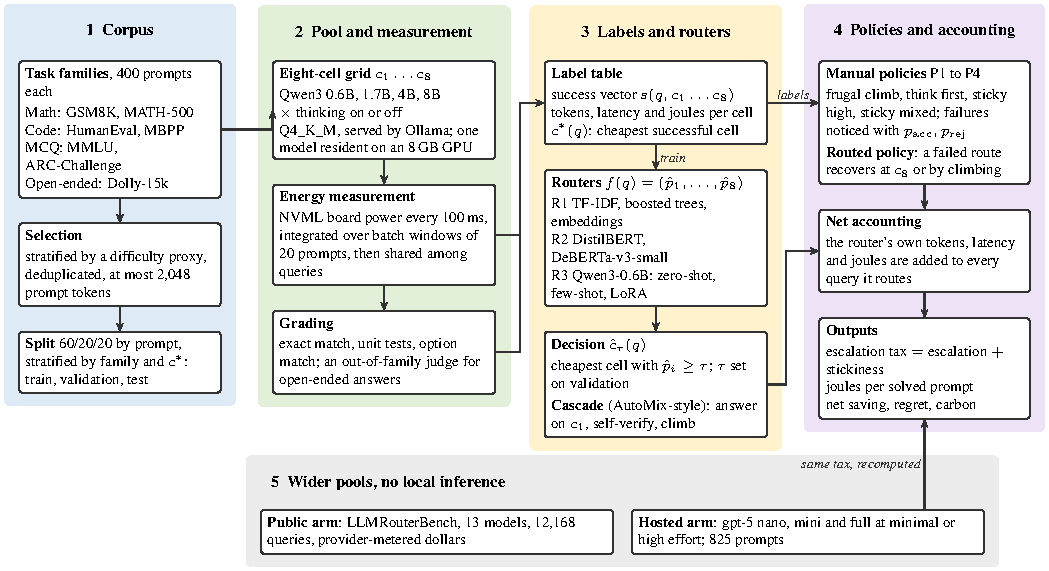
\includegraphics[width=\textwidth]{Figure_1}
\caption{Architecture of the study. Prompts from four task families (1) run
through the eight-cell grid under metered board power and are graded (2). The
grades and costs form a label table, from which routers learn the probability
that each cell succeeds and a threshold $\tau$ selects a cell (3). Manual and
routed policies are then charged by one cost function, the router's own cost
included, and yield the escalation tax and its companions (4). The public and
hosted pools reuse the policy and tax code without local inference (5).}
\label{fig:architecture}
\end{figure*}

\subsection{Configuration grid and cost}
\label{sec:grid}

The routed pool is a grid, not a ladder: four model sizes crossed with two
reasoning modes, giving eight cells $\cells = \{c_1, \dots, c_8\}$
(Table~\ref{tab:grid}). All cells come from one family, Qwen3, which offers a
size ladder in which every model runs with or without a thinking phase
\cite{qwen3}, so that size and mode are the only things that vary between
cells: tokenizer, training recipe and chat template stay the same.
Quantisation is held fixed at 4-bit (Q4\_K\_M) for the same reason, at the
cost of describing quantised models only.

\begin{table}[ht]
\centering
\caption{The eight-cell configuration grid. Sizes on disk are for the
Q4\_K\_M weights used in all experiments.}
\label{tab:grid}
\begin{tabular}{@{}cllr@{}}
\toprule
Cell & Model & Mode & Weights \\
\midrule
$c_1$ & Qwen3-0.6B & no-think & 0.52\,GB \\
$c_2$ & Qwen3-0.6B & think    & 0.52\,GB \\
$c_3$ & Qwen3-1.7B & no-think & 1.36\,GB \\
$c_4$ & Qwen3-1.7B & think    & 1.36\,GB \\
$c_5$ & Qwen3-4B   & no-think & 2.62\,GB \\
$c_6$ & Qwen3-4B   & think    & 2.62\,GB \\
$c_7$ & Qwen3-8B   & no-think & 5.23\,GB \\
$c_8$ & Qwen3-8B   & think    & 5.23\,GB \\
\bottomrule
\end{tabular}
\end{table}

We do not assume the cells are ordered by parameter count: a thinking cell of
one size can cost more than a non-thinking cell of the next size up, and
whether it does depends on the prompt. Cost is therefore measured per prompt
$q$ and per cell $c$, in three units,
\begin{align}
  \cost_{\mathrm{tok}}(c, q) &= \alpha\, n_{\mathrm{in}}(c, q)
                              + \beta\, n_{\mathrm{out}}(c, q),
  \label{eq:tokcost}\\
  \cost_{\mathrm{lat}}(c, q) &= \text{wall-clock time of the request (s)},
  \label{eq:latcost}\\
  \cost_{\mathrm{E}}(c, q)   &= \text{GPU energy of the request (J)},
  \label{eq:energycost}
\end{align}
where $n_{\mathrm{in}}$ and $n_{\mathrm{out}}$ are input and generated token
counts, the latter including any reasoning trace, and $\alpha$ and $\beta$
are per-token prices that make the token cost comparable with metered API
billing. Energy is measured, not estimated (Section~\ref{sec:energy}). All
definitions below apply to any unit; we write $\cost(c, q)$ when the unit
does not matter.

\subsection{Minimum sufficient configuration and the escalation tax}
\label{sec:tax}

Let $s(q, c) \in \{0, 1\}$ indicate whether cell $c$ produces an acceptable
answer to $q$ under the criteria of Section~\ref{sec:setup-labels}. The
\emph{minimum sufficient configuration} is the cheapest cell that succeeds,
\begin{equation}
  \cstar(q) = \argmin_{c \in \cells \,:\, s(q, c) = 1} \cost(c, q).
  \label{eq:cstar}
\end{equation}
It is undefined when no cell succeeds; those prompts are kept and reported as
the \emph{unservable fraction}, since dropping them would flatter every
policy, which pays to find out that they cannot be served.

A manual escalation policy $\pi$ consists of a starting cell and an ordered
ladder of cells to try next. The user submits $q$ to the starting cell; when
an answer is judged a failure, the \emph{whole prompt} is resubmitted to the
next rung, until an answer is accepted or the ladder runs out. With
$a_1, \dots, a_m$ the cells attempted and $a_m$ the one finally accepted, the
policy's cost is
\begin{equation}
  \mathrm{Cost}(\pi, q) = \sum\nolimits_{j=1}^{m} \cost(a_j, q).
  \label{eq:policycost}
\end{equation}
Because $n_{\mathrm{in}}$ enters \eqref{eq:tokcost} at every attempt, a long
prompt makes escalation expensive even when each failed answer is short; that
resubmission cost is absent from cascade evaluations charging only for
generated tokens. The escalation tax is the excess over the minimum
sufficient configuration,
\begin{equation}
  \Tax(\pi, q) = \mathrm{Cost}(\pi, q) - \cost\bigl(\cstar(q), q\bigr),
  \label{eq:tax}
\end{equation}
and splitting \eqref{eq:policycost} at the final attempt gives an exact
decomposition into two terms with different causes,
\begin{align}
  \Tax(\pi, q) &= \Esc(\pi, q) + \Stk(\pi, q), \label{eq:decomp}\\
  \Esc(\pi, q) &= \sum\nolimits_{j=1}^{m-1} \cost(a_j, q), \nonumber\\
  \Stk(\pi, q) &= \cost(a_m, q) - \cost\bigl(\cstar(q), q\bigr). \nonumber
\end{align}
\emph{Escalation} is the cost of attempts thrown away; \emph{stickiness} is
what the user overpays for the configuration that finally answered. When
failures are always detected, $a_m$ succeeded, so by \eqref{eq:cstar} both
components are non-negative. A user who begins on the largest thinking cell
and never moves pays only stickiness; one who climbs from the smallest cell
and stops exactly at $\cstar(q)$ pays only escalation. Most trajectories pay
some of each, and the two respond to different remedies, which is why we
report them separately.

\begin{table*}[ht]
\centering
\caption{Manual escalation policies. Cells as in Table~\ref{tab:grid}.}
\label{tab:policies}
\begin{tabularx}{\textwidth}{@{}l p{3.4cm} >{\raggedright\arraybackslash}X@{}}
\toprule
Policy & Ladder & Behaviour modelled \\
\midrule
P1 & $c_1{\to}c_3{\to}c_5{\to}c_7{\to}c_8$ & \emph{Frugal climb}: cost-conscious; larger model first, thinking last \\
P2 & $c_1{\to}c_2{\to}c_4{\to}c_6{\to}c_8$ & \emph{Think first}: turns on thinking before moving up a size \\
P3 & $c_8$ only & \emph{Sticky high}: heavyweight left selected from earlier work \\
P4 & Start drawn from an assumed distribution over cells, then the P1 ladder & \emph{Sticky mixed}: a population of users \\
\bottomrule
\end{tabularx}
\end{table*}

We construct the comparator ourselves, so we construct it generously.
Table~\ref{tab:policies} lists four policies ranging from frugal to wasteful.
P4 models a population of users who start wherever they left off; having no
usage logs, its starting distribution is an assumption, uniform over the
eight cells in the primary analysis and, as a sensitivity analysis, a
distribution in which half of all queries start at $c_8$. Both are labelled
as assumed wherever reported.

An escalating user must notice that an answer is wrong. Under \emph{oracle
detection} the user always notices and never discards a correct answer; this
regime gives the manual policies their highest solved rate and is the one we
quote in headline results. It does not bound their cost in either direction,
since rejecting a right answer adds attempts while accepting a wrong one ends
a climb early. Under \emph{imperfect detection} the user accepts a wrong
answer with probability $p_{\mathrm{acc}}$ and rejects a correct one with
probability $p_{\mathrm{rej}}$, and the last rung's answer is kept whatever
its quality. A prompt may then end unsolved, so costs are also reported per
\emph{solved} prompt,
\begin{equation}
  \bar{\cost}_{\mathrm{solved}}(\pi) =
  \frac{\mathbb{E}_q\bigl[\mathrm{Cost}(\pi, q)\bigr]}
       {\Pr_q\bigl[\text{$q$ solved under $\pi$}\bigr]}.
  \label{eq:persolved}
\end{equation}
Having no measurement of the two probabilities, we sweep them:
$p_{\mathrm{acc}} \in \{0, 0.05, 0.10, 0.15, 0.20, 0.30\}$ and
$p_{\mathrm{rej}} \in \{0, 0.05, 0.10\}$, and show
$p_{\mathrm{acc}} = 0.15$, $p_{\mathrm{rej}} = 0.05$ as an illustration.
Every outcome, including the tax and the probability of solving a prompt, is
an expectation over the user's accept-or-reject decisions, computed exactly
from the labelled success vectors rather than by simulating users.

\subsection{Routers as per-cell success predictors}
\label{sec:routers}

Every router predicts a vector of success probabilities, one per cell, rather
than a single class label,
\begin{equation}
  f(q) = \bigl(\hat{p}_1(q), \dots, \hat{p}_8(q)\bigr), \qquad
  \hat{p}_i(q) \approx \Pr\bigl[s(q, c_i) = 1\bigr],
  \label{eq:router}
\end{equation}
and a separate rule turns the vector into a decision. Given a quality
threshold $\tau \in [0, 1]$, the router picks the cheapest cell it believes
will succeed,
\begin{equation}
  \hat{c}_\tau(q) =
  \begin{cases}
    \displaystyle\argmin_{i \,:\, \hat{p}_i(q) \geq \tau} \bar{\cost}(c_i)
      & \text{if some } \hat{p}_i(q) \geq \tau,\\[1.2ex]
    \displaystyle\argmax_{i} \hat{p}_i(q) & \text{otherwise},
  \end{cases}
  \label{eq:selection}
\end{equation}
where $\bar{\cost}(c_i)$ is cell $c_i$'s mean cost on the training split,
because the true per-prompt cost is unknown before generation. Separating
prediction from decision yields a whole cost--quality curve from one trained
router by sweeping $\tau$, as Hybrid LLM exposes a quality knob at test time
\cite{ding2024hybridllm}, and lets the asymmetry between the two kinds of
error be handled by moving $\tau$ instead of retraining: routing one cell too
low produces a failure and a retry, while routing one cell too high only
wastes compute. Direct eight-way classification of $\cstar(q)$ is kept as an
ablation.

A router that picks a failing cell does not end the interaction. We charge a
routed policy as we charge a manual one: the routed cell is the first
attempt, and on failure the prompt is resubmitted once to the largest
thinking cell $c_8$. As a sensitivity analysis, a failed routed attempt
instead continues up the P1 ladder from the routed cell. The tax is then
computed with \eqref{eq:tax} exactly as for $\pi$. For each cost unit,
recovery rule and detection regime, $\tau$ is chosen on the validation split
to minimise net cost per solved prompt, router cost included, and the test
split is evaluated once at that value.

Three router families span four orders of magnitude in their own cost.
\emph{R1, classical classifiers:} logistic regression on TF-IDF word and
character $n$-grams; gradient-boosted trees
\cite{chen2016xgboost,ke2017lightgbm} on hand-built features (prompt length,
digit and operator density, code fences, question type, readability); and
logistic regression on frozen Sentence-BERT embeddings
\cite{reimers2019sbert} from all-MiniLM-L6-v2. All run
on a CPU. \emph{R2, fine-tuned encoders:} DistilBERT \cite{sanh2019distilbert}
and DeBERTa-v3-small \cite{he2023debertav3}, fine-tuned end to
end with eight sigmoid outputs, with class-weighted binary cross-entropy so
that success and failure carry equal weight in each cell. \emph{R3, a
language model as router:} Qwen3-0.6B, the smallest pool member, is shown the
eight configurations labelled A to H and asked which is the cheapest that
will answer correctly, prompted zero-shot and few-shot. Rather than decode a
letter, we read the next-token distribution at the first answer token, keep
the mass on the eight letters and renormalise, which constrains the answer to
a valid configuration and yields a distribution over $\cstar(q)$; treating
success as monotone in mean cost, $\hat{p}_i(q)$ in \eqref{eq:router} is the
mass on configurations whose mean cost does not exceed that of $c_i$. A third
variant adds LoRA adapters \cite{hu2022lora} trained to name the $\cstar$ of
each training prompt. A router larger than the models it routes between
defeats its own purpose, so we deliberately use the smallest pool member.
Because misrouting costs are asymmetric, a cost-sensitive variant of each R1
and R2 router weights errors by their realised cost consequence.

\subsection{Net-of-router accounting and the cascade baseline}
\label{sec:net}

A router is itself a workload. Each router's latency and energy per decision
are measured with the same instruments as the pool and added to the cost of
every query it routes, so that for a router $r$ and baseline policy $b$ the
\emph{net saving} is
\begin{equation}
  S_{\mathrm{net}}(r; b) =
    \mathbb{E}_q\bigl[\mathrm{Cost}(b, q)\bigr]
  - \mathbb{E}_q\bigl[\mathrm{Cost}(r, q) + \cost_{\mathrm{route}}(r, q)\bigr].
  \label{eq:netsaving}
\end{equation}
In token cost the extra term is non-zero only for R3, which consumes tokens
of its own; its decisions run through the labelling harness as short
generations and are metered per prompt exactly as the pool's are. The LoRA
variant is charged the zero-shot probe's metered cost, an upper bound, since
the probe decodes up to eight tokens where the variant needs one forward
pass. R1 and R2 decide on the CPU, which NVML cannot see, so their energy per
decision is bounded above by decision time multiplied by the upper end of the
processor's configurable power range (54\,W), and that bound is charged.

The strongest published alternative to predicting in advance is to try the
cheap configuration and check. We implement a cascade in the style of AutoMix
\cite{aggarwal2024automix}: generate on the cheapest cell, ask the same model
to verify its answer with a few-shot prompt whose four worked examples are
generic, and escalate along the P1 ladder when verification fails. The
verifier's confidence is read from a single forward pass as
$P(\text{Yes})/\bigl(P(\text{Yes}) + P(\text{No})\bigr)$ at its first answer
token, and a query escalates when that confidence falls below a threshold
chosen on the validation split, as $\tau$ is for a router. The answer from
$c_8$ is kept without verification, and AutoMix's POMDP meta-verifier is
omitted, which may weaken the cascade relative to the original method.
Verification calls are metered and charged like any other generation. This
baseline pays for failed attempts as a user does, but decides with
information from the answer itself, so beating it requires that predicting
before generation save more than that information is worth.

\subsection{Energy measurement}
\label{sec:energy}

GPU board power is read through NVIDIA's management library, NVML
\cite{nvidia_nvml}, by a sampling thread polling instantaneous power every
100\,ms. Two properties of the hardware shape the method, both established by
the telemetry gate of Section~\ref{sec:setup-gates}: the cumulative energy
counter NVML also exposes is unusable on this GPU, so energy is always
integrated from sampled power; and reported power refreshes only every 0.5\,s
and is smoothed, so a short answer from the smallest model can finish inside
one refresh period and its energy cannot be read from its own time window.

Energy is therefore integrated over \emph{batch windows}. Prompts are taken
in batches of 20, and each batch is run twice back to back on the loaded
model, once per mode, so every window holds a single cell; which mode runs
first alternates between batches. Each window is extended by a 6\,s tail after
its last generation, because reported power takes about 5\,s to decay once
generation stops, and the integral is computed with the trapezoidal rule.
Readings above 200\,W, which the GPU cannot draw under its 115\,W limit, are
discarded as read errors. We report board energy, the raw integral, and
dynamic energy, which subtracts the idle power of the GPU with the model
loaded, measured over 60\,s after warm-up and 30\,s at the end of each
session; dynamic energy is what we attribute to queries. Each query receives
a share of its window's dynamic energy in proportion to its share of the
window's generation wall time, with token share as a check. A window is
discarded and rerun, up to four times, if utilisation at the end of its tail
shows another workload or if any generation reloaded the model. Routers that
run on the GPU are measured the same way.

Two derived measures connect energy to the tax. \emph{Joules per solved
query} divides the energy a policy spends, failed attempts included, by the
number of prompts it solves, so a cheap configuration that fails and triggers
a retry is charged for the retry. \emph{Carbon} is reported as
$\mathrm{gCO_2e} = (E/3.6 \times 10^{6})\,I$ for a grid intensity $I$ in
gCO$_2$e/kWh, following Lacoste et al.\ \cite{lacoste2019quantifying} and
Luccioni et al.\ \cite{luccioni2024powerhungry}. The intensity belongs to the
grid rather than the experiment, and grids differ by more than an order of
magnitude, so carbon is reported across a bracket of intensities; the
conversion is linear, so any figure rescales.
